\documentclass{beamer}
\usepackage{graphicx}
\usepackage{amsmath}
\usepackage{kpfonts}
\usepackage{boxedminipage}
\usepackage{bcprules}
\usetheme{CambridgeUS}



\usepackage{tikz}
\usetikzlibrary{shapes,arrows}
% Define a few styles and constants
\tikzstyle{naveqs} = [draw, minimum width=10em, minimum height=5em]

%%%%%%%%%%%%%%%%Title Page%%%%%%%%%%%%%%%%%%%%%%%%%%%%%%%%%

\title[Lambda Calculus]{Introduction to Beamer}
\subtitle[]{}
\author[F. last]{Firstname Lastname}
\institute[IITB]{
  Department of Computer Science and Engineering\\
  IIT Bombay.\\
  Powai, Mumbai - 400076\\[1ex]
  \texttt{userid@cse.iitb.ac.in}
}
\date[\today]{\today}

%%%%%%%%%%%%%%%%%%%%%%%%%%%%%%%%%%%%%%%%%%%%%%%%%%%%%%%%%%%
\newtheorem{exercise}{Exercise}
\begin{document}
%--- the titlepage frame -------------------------%
\begin{frame}[plain]
  \titlepage 
\end{frame}

%%%%%%%%%%%%%%%%%%%%%%%%%%%%%%%%%%%%%%%%%%%%%%%%%%%%%%%%%%%
\begin{frame}[fragile]{\bf  This is the title}
Beamer is a \LaTeX \:class for preparing presentations.

\begin{enumerate}
\item Slides are called frames in Beamer.
\item This is the usual ordered list in \LaTeX.
\item Following slides will contain random content which will show you various ways of using it. You need to replicate it.
\item Of course! we will give you boilerplate code!
\end{enumerate}
\end{frame}
\begin{frame}[fragile]{Type Rules}
\begin{figure}
    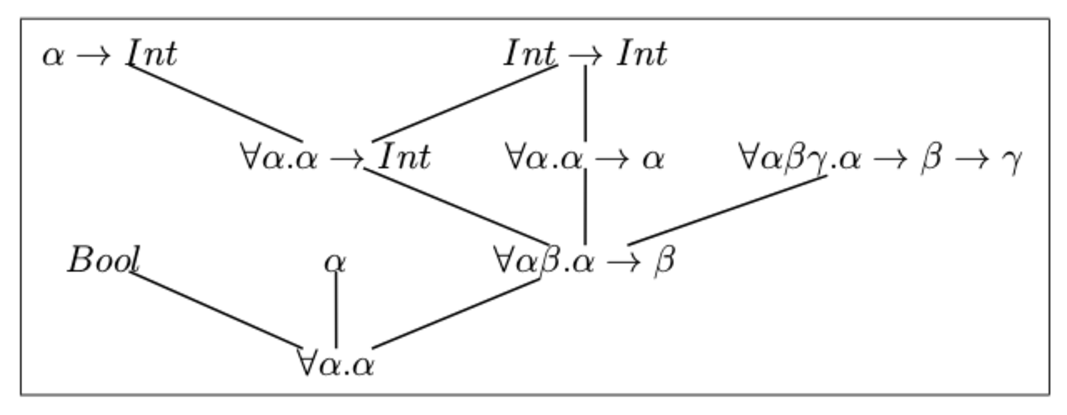
\includegraphics[width=0.8\linewidth]{type-lattice.pdf}
    \caption{This is the caption.}
    \label{Figure:}
\end{figure}
\end{frame}
\begin{frame}[fragile]{Type Rules}
\begin{itemize}
\item A substitution is a list of pairs denoted as S = \{$\alpha_1/\tau_1...\alpha_n/\tau_n$\}.
\item A substitution S applied on a type expression $\sigma$, denoted by S$\left(\sigma\right)$ involves simultaneous substitution of the variables $\alpha_1\;.\,.\,.\,\alpha_n$, if they occur free in $\sigma$, by the corresponding type expressions$\;\tau_1$ $.\,.\,.\,\tau_n$.
\begin{definition}
Let $\sigma=\forall\alpha_1\,.\,.\,.\,\alpha_m.\tau$ and $\sigma'=\forall\beta_1\,.\,.\,.\,\beta_n.\tau'$. Then $\sigma'$ is a generic
instance of $\sigma$, iff there is a substitution S acting only on $\{\alpha_1\,.\,.\,.\,\alpha_m\}$ such that $\tau'=$ S$\left(\tau\right)$ and no $\beta_i$ is free in $\sigma$.
\end{definition}
\item Clearly, the restriction that no $\beta_i$ is free in $\sigma$ is needed, else we would have absurdities like $\alpha\rightarrow Int \leq \forall\alpha.\alpha\rightarrow Int$.
\end{itemize}
\end{frame}
\begin{frame}[fragile]{\bf Recapitulation -- Type rules for $\lambda_2$}
\vspace{-0.5em}
\begin{equation}
    \Gamma\cup\{x :: \sigma\} \vdash x :: \sigma \tag{V{\scriptsize AR}}
\end{equation}
\begin{equation}
    \Gamma\cup\{c :: \sigma\} \vdash c :: \sigma \tag{C{\scriptsize ON}}
\end{equation}\vspace{-0.1em}
\begin{equation}
    \frac{\Gamma\vdash M::\sigma \;\;\;\;\;\;\;\;\; \sigma'\geq\sigma}{\Gamma\vdash M::\sigma'}\tag{I{\scriptsize NST}}
\end{equation}\vspace{-0.1em}
\begin{equation}
    \frac{\Gamma\vdash M::\sigma \;\;\;\;\;\;\;\;\; \alpha\not\in\ FV\left(\Gamma\right)}{\Gamma\vdash M::\forall\alpha.\sigma}\tag{{\large G}{\scriptsize EN}}
\end{equation}\vspace{-0.1em}
\begin{equation}
    \frac{\Gamma\vdash M::\tau_1\rightarrow\tau_2 \;\;\;\;\;\;\;\;\; \Gamma\vdash N::\tau_1}{\Gamma\vdash M::\sigma'}\tag{M-A{\scriptsize PP}}
\end{equation}\vspace{-0.1em}
\begin{equation}
    \frac{\Gamma,x ::\tau_1\vdash M ::\tau_2}{\Gamma\vdash \lambda x.M::\tau_1\rightarrow\tau_2}\tag{M-A{\scriptsize BS}}
\end{equation}
\end{frame}
\begin{frame}[fragile]{\bf Hindley-Milner - Type checking variables}
\begin{enumerate}
    \item[1:] \textbf{$t$ is a variable} $x$ 
    \begin{center}
    \begin{tikzpicture}[node distance=2.5cm,auto,>=latex']
    \node (naveq) [naveqs] {$x$};
    \path (naveq.south)+(0.0,-0.5) node (s1) {\footnotesize $\Gamma\;x=\forall\alpha_1,...\alpha_n\cdot\tau$};
    \path (naveq.east)+(2.1,0.8) node (s2) {\scriptsize {$\tau\left[\alpha_1/\beta_1,\,.\,.\,.\,\alpha_n/\beta_n\right],\;\beta_1,\,.\,.\,.\,\beta_n\!\!\!\not\in\!\!\Gamma$}};
    \path (naveq.west)+(-2,0.4) node (s2) {\footnotesize $\:\Gamma$};
    \path (naveq.east)+(2,-0.8) node (s3) {\scriptsize The identity substitution $\theta_i_d$};
    \draw [->,thick] (naveq.east)+(0,-0.5) -- (3.5,-0.5);
    \draw [->,thick] (naveq.east)+(0,0.5) -- (3.5,0.5);
    \draw [->,thick] (-3.5,0) -- (naveq.west);
    \end{tikzpicture}
    \end{center}
    \begin{itemize}
        \item $\beta_1,\,.\,.\,.\,,\beta_n$ are fresh variables.
        \item Reason for monomorphising the type of $x$: We try to find the type of a variable only in the context of an application, and our application is monomorphic.
    \end{itemize}
\end{enumerate}
\end{frame}
\begin{frame}[fragile]{\bf Hindley-Milner - Type checking applications}
\begin{enumerate}
\item[1] Typecheck $e_1$ with the initial environment $\Gamma$. Result is $\tau_1$ and $\theta_1$.
\item[2] Typecheck $e_2$ with the environment $\theta_1\Gamma$. Result is $\tau_2$ and $\theta_2$.
\item[3] Unify $\theta_2\:\tau_1$ and $\tau_2\rightarrow\alpha$. Assume that unifier is $\theta$. And the unified term $\left(\theta\;\alpha\right)$ is $\tau_3$.
\item[4] Type of the application is $\tau_3$ and the final substitution is $\theta\circ\theta_2\circ\theta_1$.
\end{enumerate}
\end{frame}
\end{document}
